\documentclass[10pt,twocolumn]{article}

\usepackage[margin=0.72in]{geometry}
\usepackage{amsmath,amssymb,bm}
\usepackage{booktabs}
\usepackage{graphicx}
\usepackage{xcolor}
\usepackage{url}
\usepackage[colorlinks=true,allcolors=blue]{hyperref}

\graphicspath{{../results/paper_assets/}}

\newcommand{\method}{One-sided $\Delta$-Physics}
\newcommand{\nuRef}{\nu_0}
\newcommand{\RelLtwo}{\mathrm{RelL2}}
\newcommand{\PSRE}{\mathrm{PSRE}}

\title{One-sided $\Delta$-Physics: Zero-Shot Viscosity Adaptation of Frozen Neural Time-Steppers}
\author{Author Name\\Institution\\\texttt{email@example.com}}
\date{}

\begin{document}
\maketitle



\begin{abstract}
Neural PDE time-steppers can achieve efficient surrogate
simulation, but their accuracy often deteriorates under
unseen physical parameter shifts, particularly during
long autoregressive rollouts. We propose
\textbf{One-sided $\Delta$-Physics}, a lightweight
analytical framework for zero-shot adaptation of
pretrained neural time-steppers to higher-viscosity
regimes. Rather than learning parameter dependence
from additional simulations, our method corrects
a frozen reference predictor using the difference
between the target and reference dissipative
semigroups. A one-sided policy activates the
correction only when the target viscosity exceeds
the reference viscosity, avoiding potentially
anti-dissipative adjustments. The method requires
no target-parameter training data, retraining,
or additional learned parameters, and retains
one neural-network evaluation per physical step.
We evaluate the approach on two-dimensional
Navier--Stokes and one-dimensional viscous Burgers
equations. At twice the reference viscosity,
Step-50 relative $L_2$ errors are reduced by
$22.19\%$ and $91.87\%$, respectively.
Spectral analysis further demonstrates substantial
reductions in dissipative mismatch. Comparisons
with multi-viscosity supervision and iterative
adaptation highlight the method's favorable
data and inference efficiency, establishing
a practical approach to zero-shot adaptation
when target-parameter simulations are unavailable.
\end{abstract}


\section{Introduction}
\label{sec:introduction}

Partial differential equations (PDEs) describe the evolution of physical systems ranging from fluid flows to transport and diffusion processes. Accurate numerical simulation can be expensive when solutions are repeatedly required for different initial conditions and physical parameters. Neural operators offer an alternative by learning mappings between function spaces from data \cite{lu2021deeponet,kovachki2023neuraloperator}. In particular, Fourier Neural Operators (FNOs) use spectral transformations for efficient global information exchange \cite{li2021fno}, while Factorized Fourier Neural Operators (F-FNOs) employ separable spectral operations and residual architectures to improve their efficiency and predictive performance \cite{tran2023ffno}.

Despite these advances, a neural time-stepper trained under one set of physical parameters may not generalize reliably to another. Parameter shifts can change both the evolution of physical structures and their spatial frequency content \cite{gupta2023multiscale}. The difficulty is amplified during autoregressive prediction, where errors are fed back into subsequent steps. Prior studies have identified the importance of accurately representing non-dominant frequency components for long rollouts \cite{lippe2023pderefiner}, and systematic benchmarks emphasize that short-horizon accuracy alone is insufficient to characterize neural PDE emulators \cite{koehler2024apebench}.

One route to improved generalization is to learn across a broader range of governing dynamics, through parameter conditioning, multi-environment adaptation, or multi-physics pretraining \cite{gupta2023multiscale,kirchmeyer2022coda,koupai2024geps,mccabe2024mpp,herde2024poseidon}. Physical knowledge can also be incorporated during training, for example through governing-equation constraints \cite{li2024pino}. However, training at multiple parameter values or adapting a learned context to a new environment may be costly or infeasible when only simulations at a single reference parameter are available.

More recent approaches reuse pretrained operators at test time. Neural Operator Splitting searches over compositions of learned dynamics using observations from the target system \cite{serrano2026splitting}, while MD-PNOP and Equation Recast exploit known differences between governing equations to reuse a reference operator through analytical reformulation and iterative solution procedures \cite{cheng2026mdpnop,cheng2026recast}. These developments suggest a narrower question for dissipative autoregressive surrogates: \emph{if a parameter changes a known linear dissipative term, can that change be incorporated directly into a frozen time-stepper without target-trajectory calibration, operator search, or iterative neural inference?}

We address this question with \textbf{One-sided $\Delta$-Physics}, a lightweight analytical correction for adapting a reference-viscosity neural time-stepper to unseen higher viscosities. The method adds the known difference between target and reference dissipative semigroups to the frozen prediction, and bypasses the correction when the target viscosity is no larger than the reference value. It requires no target-parameter training data, retraining, or additional learned parameters, while retaining one neural-network evaluation per physical step. Experiments on Navier--Stokes and viscous Burgers equations demonstrate improvements in long-horizon prediction and spectral accuracy, and clarify the accuracy--cost tradeoff relative to supervised conditioning and iterative adaptation.

Our contributions are threefold:
\begin{itemize}
    \item We introduce a \textbf{one-shot, zero-shot analytical correction} that transfers a frozen neural time-stepper to higher-viscosity regimes using a known linear dissipative operator.

    \item We develop a \textbf{dissipation-aware one-sided policy}, motivated by the sign of the semigroup difference and supported by viscosity-sweep ablations, without claiming a global stability guarantee for the full learned dynamics.

    \item We demonstrate \textbf{cross-PDE long-rollout and spectral improvements} with no additional learned parameters and low test-time overhead, and characterize the tradeoff against data-intensive and iterative alternatives.
\end{itemize}


\section{Related Work}
\label{sec:related_work}

\subsection{Neural and Spectral Operators for PDE Dynamics}

Fourier-based neural operators learn global transformations efficiently in the frequency domain. FNO established a spectral operator-learning architecture for parametric PDEs \cite{li2021fno}, and F-FNO improved its representation through dimension-wise factorization and residual stacking \cite{tran2023ffno}. More recent methods address limitations of fixed or truncated spectral representations in different ways. Point-Calibrated Spectral Neural Operators adapt spectral bases to pointwise frequency preferences \cite{yue2024pcsm}; FreqMoE progressively extends learned low-frequency information to higher-frequency components using sparse experts \cite{chen2025freqmoe}; and TF-SNO uses state-dependent time--frequency gates to modulate spectral responses during non-stationary evolution \cite{zhou2026tfsno}.

Reliable temporal prediction is a related but distinct challenge. PDE-Refiner uses a learned multistep denoising procedure to better recover low-amplitude spectral information that can influence long rollouts \cite{lippe2023pderefiner}. APEBench formalizes evaluation across autoregressive emulators and emphasizes rollout-dependent comparisons \cite{koehler2024apebench}. These methods primarily develop neural representations, training procedures, or learned refinement mechanisms. By contrast, our correction is determined by the known change in a PDE coefficient and acts outside a previously trained time-stepper, without altering its spectral weights or adding learned gates.

\subsection{Generalization Across PDE Parameters}

A common strategy for parametric PDEs is to expose a surrogate to multiple parameter settings during training. Gupta and Brandstetter examine the effects of parameter and temporal-scale conditioning on neural PDE architectures \cite{gupta2023multiscale}. Multiple Physics Pretraining and Poseidon pursue transfer through training on broader collections of physical systems \cite{mccabe2024mpp,herde2024poseidon}. Such methods broaden the experience of a learned surrogate, but their supervision requirements differ from a model trained at a single reference viscosity.

Other approaches adapt a pretrained or shared dynamics model from limited observations of a new environment. CoDA learns a shared dynamics model and a low-dimensional context-dependent parameterization, adapting the context using observations from the new system \cite{kirchmeyer2022coda}. GEPS improves the scalability of this idea through low-rank adaptive conditioning and first-order context optimization \cite{koupai2024geps}. Zhu et al. investigate neural-operator extrapolation more broadly, including shifts in the distribution of input functions, and improve predictions using physics-based fine-tuning or sparse observations and multifidelity learning \cite{zhu2023extrapolation}. These studies show the value of target information and efficient adaptation, whereas our setting assumes that the target viscosity is known but that no target-parameter trajectory is available for adaptation or parameter updates.

\subsection{Physics-Guided and Structure-Preserving Correction}

Physical knowledge can be integrated into the learning objective or into a numerical solver. Physics-informed DeepONets and PINO use governing-equation residuals to constrain learned solution operators \cite{wang2021physicsdeeponet,li2024pino}. Hybrid approaches couple learned components with numerical simulation: Solver-in-the-Loop trains learned corrections through differentiable solver rollouts \cite{um2020solverintheloop}, while machine-learning-accelerated computational fluid dynamics incorporates learned components into a traditional CFD discretization \cite{kochkov2021mlcfd}. These approaches generally alter the training or solver pipeline rather than applying a fixed analytical correction to an independently trained surrogate.

Post-training or structural correction is particularly relevant to our work. McGreivy and Hakim modify learned time updates to enforce discrete physical invariants, such as conservation and norm constraints \cite{mcgreivy2023invariants}. Li et al. study learned evolution operators for dissipative chaotic systems, including dissipativity-promoting regularization and post-processing \cite{li2022chaotic}. Deep-OSG instead incorporates the semigroup composition property into the training of a family of learned flow maps with varying time increments \cite{chen2023deeposg}. In classical numerical analysis, exponential integrators exploit the known exponential evolution of linear operators, particularly for stiff and parabolic problems \cite{hochbruck2010exponential}. Our approach builds on this established mathematical structure but uses it for a different purpose: a \emph{difference of linear dissipative semigroups across parameter values} is added at inference time to a frozen neural prediction. This property characterizes the analytical correction, not the stability of the complete nonlinear rollout.

\subsection{Zero-Shot Test-Time Adaptation}

A more direct point of comparison is test-time reuse of learned operators in previously unseen regimes. DISCO uses trajectory context to generate an evolution operator with a hypernetwork \cite{morel2025disco}. Building on this operator-discovery framework, Neural Operator Splitting constructs a dictionary of learned dynamics and searches at test time for operator compositions that explain a short observed target trajectory; selected operators are subsequently combined using splitting schemes \cite{serrano2026splitting}. This route enables adaptation without updating pretrained weights, but requires a suitable operator dictionary and target-system observations for search.

Equation-based recasting offers another approach to extrapolation. MD-PNOP exploits differences between governing operators to formulate reference-operator problems and combines neural predictions with iterative numerical-solver refinement \cite{cheng2026mdpnop}. Equation Recast develops canonical-operator reuse by absorbing parameter-induced operator differences into effective source terms and iteratively solving the resulting recast equations \cite{cheng2026recast}; its applications include both steady PDEs and time-dependent problems. Thus, analytical parameter transfer and test-time zero-shot reuse are not new in themselves.

One-sided $\Delta$-Physics targets the more specific case of an autoregressive neural time-stepper trained at a single reference viscosity with a known linear dissipative term. Instead of inferring a target operator from trajectory context or iteratively resolving an effective source, we apply a predetermined semigroup-difference correction in one step. This separates our contribution from prior operator composition, invariant-preserving post-processing, and equation-recasting approaches: the adaptation uses a known viscosity shift, no target-trajectory calibration, no new learned module, and only one neural evaluation per physical time step.



\section{Method}
\label{sec:method}

We consider time-dependent dissipative PDEs whose dynamics can be written as
\begin{equation}
    \partial_t u
    =
    \nu \mathcal{L}u
    +
    \mathcal{N}(u),
    \label{eq:pde_general}
\end{equation}
where $u$ denotes the evolving state, $\nu>0$ is a physical parameter controlling
the strength of dissipation, $\mathcal{L}$ is a known linear dissipative operator,
and $\mathcal{N}$ collects the remaining nonlinear dynamics and forcing terms.
For the viscous Burgers and Navier--Stokes equations considered in this work,
$\mathcal{L}=\Delta$ is the Laplacian. For Navier--Stokes in vorticity form,
$u=\omega$.

Our goal is to train a neural time-stepper only at a single reference viscosity
$\nu_0$, and then adapt the frozen model at inference time to previously unseen
higher viscosities $\nu>\nu_0$, without target-viscosity trajectories,
parameter updates, or additional learned modules.

\subsection{Reference Increment Time-Stepper}
\label{sec:reference_stepper}

Let $\Delta t$ denote the physical time interval between two consecutive states
used for supervised learning. We train a neural operator at the reference
viscosity $\nu_0$ to predict the state increment,
\begin{equation}
    F_\theta(u_t)
    \approx
    u_{t+\Delta t}-u_t.
\end{equation}
The resulting one-step predictor is
\begin{equation}
    \Phi_{\theta,\nu_0}(u_t)
    =
    u_t + F_\theta(u_t).
    \label{eq:increment_model}
\end{equation}
In our Navier--Stokes experiments, $F_\theta$ is implemented using an
F-FNO backbone, while the one-dimensional Burgers experiments use an FNO
backbone. The proposed correction is independent of the particular neural
operator architecture.

After training, $\theta$ is frozen. Importantly, because the model is trained
on trajectories generated at $\nu_0$, the learned time-stepper already contains
the reference-viscosity dissipative dynamics. Therefore, adding the full
target-viscosity diffusion operator on top of
$\Phi_{\theta,\nu_0}$ would generally double-count the dissipation already
encoded in the learned predictor. We instead correct only the analytically known
\emph{difference} between the target and reference dissipative dynamics.

\subsection{Analytical Semigroup Difference}
\label{sec:semigroup_difference}

Consider first the known linear dissipative component of
Eq.~\eqref{eq:pde_general},
\begin{equation}
    \partial_t u = \nu \mathcal{L}u.
\end{equation}
Its exact evolution over one time interval $\Delta t$ is given by the
linear semigroup
\begin{equation}
    S_\nu
    =
    \exp\!\left(\nu \Delta t\,\mathcal{L}\right).
    \label{eq:semigroup_general}
\end{equation}
The change in the linear evolution induced by replacing the reference
viscosity $\nu_0$ with a target viscosity $\nu$ is therefore
\begin{equation}
    C_{\nu,\nu_0}(u_t)
    =
    \left(S_\nu-S_{\nu_0}\right)u_t.
    \label{eq:delta_correction_general}
\end{equation}

For periodic diffusion with $\mathcal{L}=\Delta$, the correction can be evaluated
analytically in Fourier space. Let $\widehat{u}(\bm{k})=\mathcal{F}[u](\bm{k})$,
where $\bm{k}$ denotes the physical wavenumber. Then
\begin{equation}
    S_\nu u
    =
    \mathcal{F}^{-1}
    \left[
        e^{-\nu |\bm{k}|^2\Delta t}
        \widehat{u}(\bm{k})
    \right],
    \label{eq:diffusion_semigroup}
\end{equation}
and hence
\begin{equation}
    C_{\nu,\nu_0}(u_t)
    =
    \mathcal{F}^{-1}
    \left[
        \left(
        e^{-\nu |\bm{k}|^2\Delta t}
        -
        e^{-\nu_0 |\bm{k}|^2\Delta t}
        \right)
        \widehat{u_t}(\bm{k})
    \right].
    \label{eq:delta_fourier}
\end{equation}
For a periodic domain with side length $\ell_j$ along dimension $j$, the
physical wavenumbers are $k_j=2\pi n_j/\ell_j$.

Equation~\eqref{eq:delta_fourier} is the central analytical component of our
method. Rather than asking the neural operator to infer the entire
viscosity dependence from data, we retain the learned reference dynamics and
supply the known linear parameter shift directly from the governing equation.

\subsection{One-Sided \texorpdfstring{$\Delta$}{Delta}-Physics}
\label{sec:one_sided_delta}

A symmetric use of Eq.~\eqref{eq:delta_correction_general} is not equally
well behaved on both sides of the reference viscosity. For
$\nu>\nu_0$, the target system is more dissipative than the reference system,
and the semigroup difference supplies additional attenuation. In contrast,
for $\nu<\nu_0$, the semigroup difference reverses sign and acts as an
anti-dissipative correction.

We therefore introduce a one-sided policy,
\begin{equation}
    C^{+}_{\nu,\nu_0}(u_t)
    =
    \mathbf{1}_{\{\nu>\nu_0\}}
    \left(S_\nu-S_{\nu_0}\right)u_t,
    \label{eq:onesided_correction}
\end{equation}
where $\mathbf{1}_{\{\nu>\nu_0\}}$ is an indicator function. The final
One-sided $\Delta$-Physics predictor is
\begin{equation}
    \boxed{
    \Phi^\Delta_{\nu}(u_t)
    =
    \Phi_{\theta,\nu_0}(u_t)
    +
    C^{+}_{\nu,\nu_0}(u_t)
    }
    \label{eq:delta_physics_final}
\end{equation}
or, equivalently,
\begin{equation}
    \Phi^\Delta_{\nu}(u_t)
    =
    \begin{cases}
        u_t+F_\theta(u_t),
        & \nu\le\nu_0,
        \\[2mm]
        u_t+F_\theta(u_t)
        +
        (S_\nu-S_{\nu_0})u_t,
        & \nu>\nu_0.
    \end{cases}
    \label{eq:delta_physics_piecewise}
\end{equation}

The correction is applied at every autoregressive step. Thus, for a rollout
initialized from $u_0$,
\begin{equation}
    \widehat{u}_{t+\Delta t}
    =
    \Phi^\Delta_{\nu}(\widehat{u}_t),
\end{equation}
and the corrected prediction is recursively fed into the next step.

The name $\Delta$-Physics refers to the use of a \emph{difference in known
physics} between the target and reference parameter regimes:
$S_\nu-S_{\nu_0}$. The structure is shown in Figure~\ref{fig:method}.

\begin{figure*}[t]
    \centering
    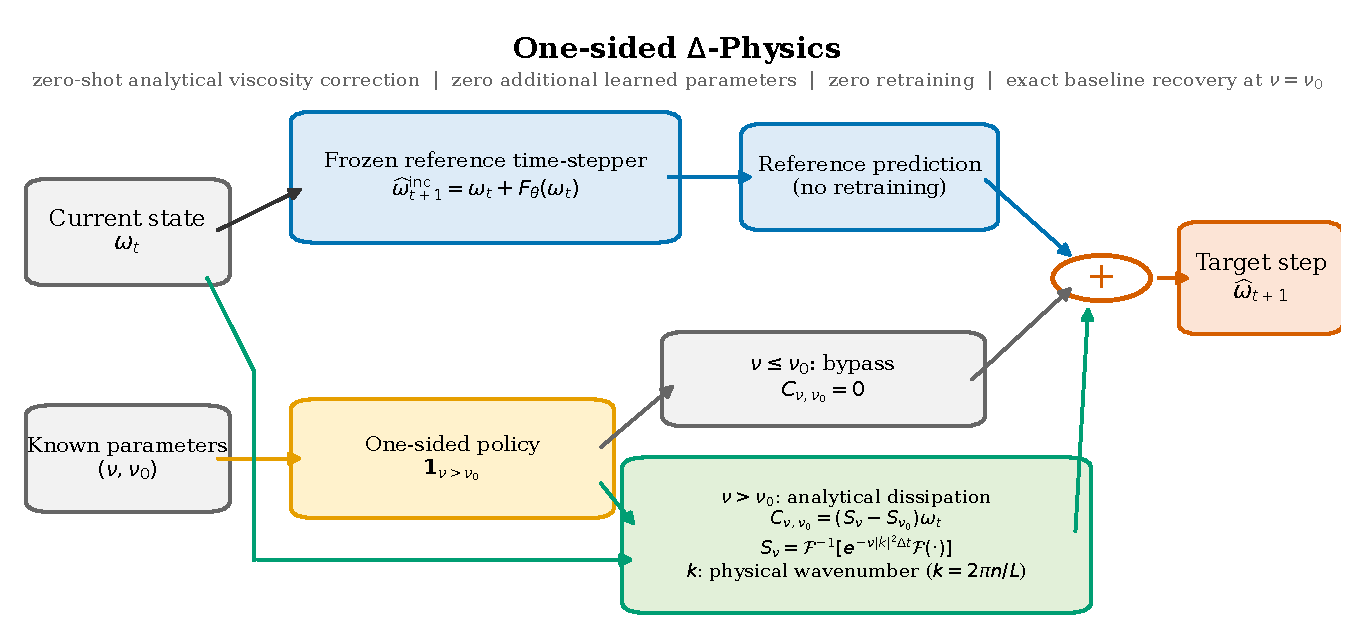
\includegraphics[width=0.98\textwidth]{figure_1_method.pdf}
    \caption{Overview of One-sided $\Delta$-Physics. The current state $u_t$
    is passed to both the frozen reference time-stepper and the analytical
    semigroup-difference correction. The known parameters $(\nu,\nu_0)$
    determine whether the correction is activated. For $\nu\leq\nu_0$, the
    correction is bypassed; for $\nu>\nu_0$, the dissipative correction
    $(S_\nu-S_{\nu_0})u_t$ is added to the frozen Increment prediction. The
    construction introduces zero additional learned parameters and exactly
    recovers the reference predictor at $\nu=\nu_0$.}
    \label{fig:method}
\end{figure*}

\subsection{Dissipative Property}
\label{sec:dissipative_property}

The one-sided design admits a simple stability-motivated interpretation.
Assume that $\mathcal{L}$ is self-adjoint and negative semidefinite, as is the
Laplacian under periodic boundary conditions. Let
$\{\lambda_j\}$ denote its eigenvalues, with $\lambda_j\le0$.
For $\nu\ge\nu_0$,
\begin{equation}
    e^{\nu\Delta t\lambda_j}
    -
    e^{\nu_0\Delta t\lambda_j}
    \le 0.
\end{equation}
Therefore,
\begin{equation}
    \left\langle
        u,
        (S_\nu-S_{\nu_0})u
    \right\rangle
    \le 0,
    \qquad
    \nu\ge\nu_0.
    \label{eq:dissipative_inner_product}
\end{equation}

For the periodic Laplacian, this follows directly from Parseval's identity:
\begin{align}
    \left\langle
        u,
        (S_\nu-S_{\nu_0})u
    \right\rangle
    &=
    \sum_{\bm{k}}
    \left(
        e^{-\nu|\bm{k}|^2\Delta t}
        -
        e^{-\nu_0|\bm{k}|^2\Delta t}
    \right)
    |\widehat{u}(\bm{k})|^2
    \nonumber\\
    &\le 0,
    \qquad \nu\ge\nu_0.
    \label{eq:dissipative_fourier}
\end{align}

Hence, in the activated regime, the analytical correction has a non-positive
Fourier multiplier at every mode. This characterizes the dissipative direction
of the correction, but does not guarantee energy decay or global stability of
the complete neural predictor. Conversely, when $\nu<\nu_0$, the sign of the
multiplier reverses, yielding an anti-dissipative correction. This motivates
the one-sided policy in Eq.~\eqref{eq:onesided_correction}.

We emphasize that Eq.~\eqref{eq:dissipative_inner_product} characterizes the
analytical correction alone and does not constitute a global stability guarantee
for the full nonlinear neural rollout.

\subsection{Reference Recovery and Linear Exactness}
\label{sec:reference_recovery}

The proposed correction preserves the original reference model exactly. At
$\nu=\nu_0$,
\begin{equation}
    S_\nu-S_{\nu_0}=0,
\end{equation}
so that
\begin{equation}
    \Phi^\Delta_{\nu_0}(u_t)
    =
    \Phi_{\theta,\nu_0}(u_t).
    \label{eq:exact_reference_recovery}
\end{equation}
Thus, applying $\Delta$-Physics cannot alter the baseline prediction at the
reference viscosity.

The correction is also exact for the purely linear dissipative problem in the
activated regime. If $\mathcal{N}=0$ and the reference predictor is exact,
such that
\begin{equation}
    \Phi_{\theta,\nu_0}(u_t)=S_{\nu_0}u_t,
\end{equation}
then for $\nu>\nu_0$,
\begin{align}
    \Phi^\Delta_\nu(u_t)
    &=
    S_{\nu_0}u_t
    +
    (S_\nu-S_{\nu_0})u_t
    \nonumber\\
    &=
    S_\nu u_t.
\end{align}
For nonlinear PDEs, however, viscosity changes can also alter the nonlinear
trajectory itself. Our method does not attempt to learn or approximate this
unknown nonlinear parameter shift. It corrects only the analytically known
change in the linear dissipative evolution. 

\subsection{Training and Inference Cost}
\label{sec:complexity}

One-sided $\Delta$-Physics requires no modification of the training procedure.
The reference neural operator is trained using data from $\nu_0$ only, and no
samples from the target viscosity are required. At test time, all neural-network
parameters remain frozen.

For $\nu>\nu_0$, each physical time step requires
\begin{enumerate}
    \item one forward evaluation of the reference neural time-stepper;
    \item one analytical semigroup-difference evaluation using FFTs and
    element-wise spectral multiplication.
\end{enumerate}
The correction introduces no additional learned parameters and requires no
test-time optimization or fixed-point iteration. For a grid containing $N$
degrees of freedom, the analytical correction has complexity
$\mathcal{O}(N\log N)$ due to the Fourier transforms, while the number of neural
network evaluations remains exactly one per physical step. When
$\nu\le\nu_0$, the correction is bypassed and inference reduces exactly to the
original reference model.

This yields a different operating regime from multi-parameter supervised
models, which can achieve higher accuracy when target-parameter trajectories
are available but require additional parameter coverage during training.
One-sided $\Delta$-Physics instead targets the zero-shot setting in which only
reference-viscosity data are available and adaptation must be performed without
retraining.

\section{Experiments}
\label{sec:experiments}

We evaluate One-sided $\Delta$-Physics on two dissipative PDEs, namely, 
two-dimensional forced Navier--Stokes in vorticity form and the
one-dimensional viscous Burgers equation. Our experiments are designed to
answer five questions:
(i) whether the analytical correction improves zero-shot adaptation to unseen
higher viscosities;
(ii) whether the benefit increases with viscosity shift and rollout horizon;
(iii) whether the same behavior transfers across PDEs and neural-operator
backbones;
(iv) whether the improvement is consistent with the intended spectral
dissipation mechanism; and
(v) how the proposed one-shot correction compares with stronger alternatives
that use either additional parameter-specific training data or additional
test-time computation.

\subsection{Experimental Setup}
\label{sec:experimental_setup}

\paragraph{Navier--Stokes.}
We consider the two-dimensional incompressible Navier--Stokes equation in
vorticity form on the periodic unit square,
\begin{equation}
    \partial_t \omega
    +
    \mathbf{v}\cdot\nabla\omega
    =
    \nu \Delta\omega + f,
    \label{eq:ns_exp}
\end{equation}
where $\omega$ is the vorticity, $\mathbf{v}$ is the velocity recovered from
the stream function, and $\nu$ is the viscosity. We use the fixed forcing
\begin{equation}
    f(x,y)
    =
    0.1\left[
    \sin\!\left(2\pi(x+y)\right)
    +
    \cos\!\left(2\pi(x-y)\right)
    \right].
    \label{eq:ns_forcing}
\end{equation}
Spatial derivatives are evaluated spectrally, with dealiasing applied to the
nonlinear advection term. Ground-truth trajectories are integrated with
fourth-order Runge--Kutta using an internal solver step
$\delta t=0.005$, while consecutive states supplied to the neural
time-stepper are separated by
\begin{equation}
    \Delta t = 0.05.
\end{equation}

The main Navier--Stokes experiments use a $64\times64$ grid and a reference
viscosity
\begin{equation}
    \nu_0 = 10^{-3}.
\end{equation}
For each independent seed, we generate 24 training trajectories and
6 validation trajectories at $\nu_0$. Each training trajectory contains
20 one-step transitions, giving 480 training pairs. Evaluation uses
8 independent trajectories per viscosity and 50-step free-running
autoregressive rollouts. The main high-viscosity evaluation considers
\begin{equation}
    \frac{\nu}{\nu_0}
    \in
    \{1.0,1.5,1.75,2.0\}.
\end{equation}
For a fixed seed, the same initial conditions are used across test
viscosities, so differences between viscosity settings are not confounded by
different initial states.

The reference model is an F-FNO with width 16, eight retained modes per
factorized Fourier branch, eight residual layers, and feed-forward expansion
factor 4. Fourier weights are shared across depth. The input consists of the
normalized vorticity field and the two spatial coordinates. The resulting
reference model contains 28,370 learned parameters.

\paragraph{Viscous Burgers.}
To test whether the correction transfers beyond Navier--Stokes, we consider
the one-dimensional viscous Burgers equation
\begin{equation}
    \partial_t u
    +
    u\,\partial_x u
    =
    \nu\,\partial_{xx}u
    \label{eq:burgers_exp}
\end{equation}
on the periodic unit interval. Ground-truth trajectories are generated using
spectral spatial derivatives, dealiasing of the nonlinear term, and
fourth-order Runge--Kutta integration. The internal integration step is
$\delta t=0.002$, and consecutive neural-operator states are separated by
\begin{equation}
    \Delta t = 0.02.
\end{equation}

We use 64 spatial grid points and reference viscosity
\begin{equation}
    \nu_0 = 10^{-2}.
\end{equation}
As for Navier--Stokes, each seed uses 24 training trajectories,
6 validation trajectories, and 8 test trajectories per viscosity, with
20 transitions per training trajectory and 50-step free-running evaluation.
We evaluate
\begin{equation}
    \frac{\nu}{\nu_0}
    \in
    \{1.0,1.25,1.5,1.75,2.0\}.
\end{equation}

Because the dimensional factorization used by F-FNO degenerates to a single
Fourier direction in one spatial dimension, we use a standard FNO1d
backbone for Burgers. The model has width 32, 16 retained Fourier modes,
and four Fourier layers, with pointwise residual transformations in each
layer. The same One-sided $\Delta$-Physics correction is applied without
modification to the correction formula.

\paragraph{Training protocol.}
Both reference models are trained to predict normalized state increments
rather than absolute next states. Input states and target increments are
normalized using statistics computed from the training set only. We minimize
mean squared error on the normalized increments using Adam with learning rate
$10^{-3}$, weight decay $10^{-6}$, and batch size 32. All models are trained
for 15 epochs. A StepLR scheduler with decay factor $0.5$ is applied with
step size $\lfloor 15/2\rfloor$. The checkpoint with the lowest validation
one-step relative $L_2$ error is retained.

All formal results are reported over three independent seeds,
\begin{equation}
    s\in\{0,1,2\},
\end{equation}
as mean $\pm$ sample standard deviation. During evaluation, predictions are
generated recursively without teacher forcing.

\paragraph{Evaluation metrics.}
Our primary metric is relative $L_2$ error. For a prediction
$\widehat{u}$ and target $u$, we write
\begin{equation}
    E_{\mathrm{RelL2}}
    =
    \frac{\|\widehat{u}-u\|_2}
         {\|u\|_2}.
    \label{eq:rell2_metric}
\end{equation}
We report errors at selected rollout horizons as well as their average over
the complete 50-step rollout, denoted Avg-50 RelL2.

Because the proposed correction acts directly on the dissipative Fourier
dynamics, we additionally measure the relative error of the power spectrum.
Let
\begin{equation}
    P_{\widehat{u}}(\mathbf{k})
    =
    |\mathcal{F}[\widehat{u}](\mathbf{k})|^2,
    \qquad
    P_u(\mathbf{k})
    =
    |\mathcal{F}[u](\mathbf{k})|^2.
\end{equation}
We define the power-spectrum relative error (PSRE) as
\begin{equation}
    E_{\mathrm{PSRE}}
    =
    \frac{
        \|P_{\widehat{u}}-P_u\|_2
    }{
        \|P_u\|_2
    }.
    \label{eq:psre_metric}
\end{equation}
We report both the average PSRE over the 50-step rollout and the final-step
PSRE.

For improvement plots, the paired relative improvement of
One-sided $\Delta$-Physics over the Increment baseline is
\begin{equation}
    \mathrm{Improvement}
    =
    100
    \times
    \frac{
        E_{\mathrm{Increment}}
        -
        E_{\Delta\text{-Physics}}
    }{
        E_{\mathrm{Increment}}
    }.
    \label{eq:improvement_metric}
\end{equation}
Improvements are first computed within each seed and are then summarized
across the three seeds.

\subsection{Zero-Shot Adaptation on
\texorpdfstring{$64\times64$}{64x64} Navier--Stokes}
\label{sec:ns_results}

We first evaluate whether a model trained exclusively at the reference
viscosity can be adapted to unseen, more dissipative regimes without
retraining. Figure~\ref{fig:cross_pde}(a) shows the relative improvement of
One-sided $\Delta$-Physics over the frozen Increment F-FNO at different
viscosity ratios and rollout horizons. Absolute errors and spectral metrics
are reported in Table~\ref{tab:ns64_main}, with complete horizon-wise results
provided in Table~\ref{tab:ns64_absolute}.

\begin{figure*}[t]
    \centering
    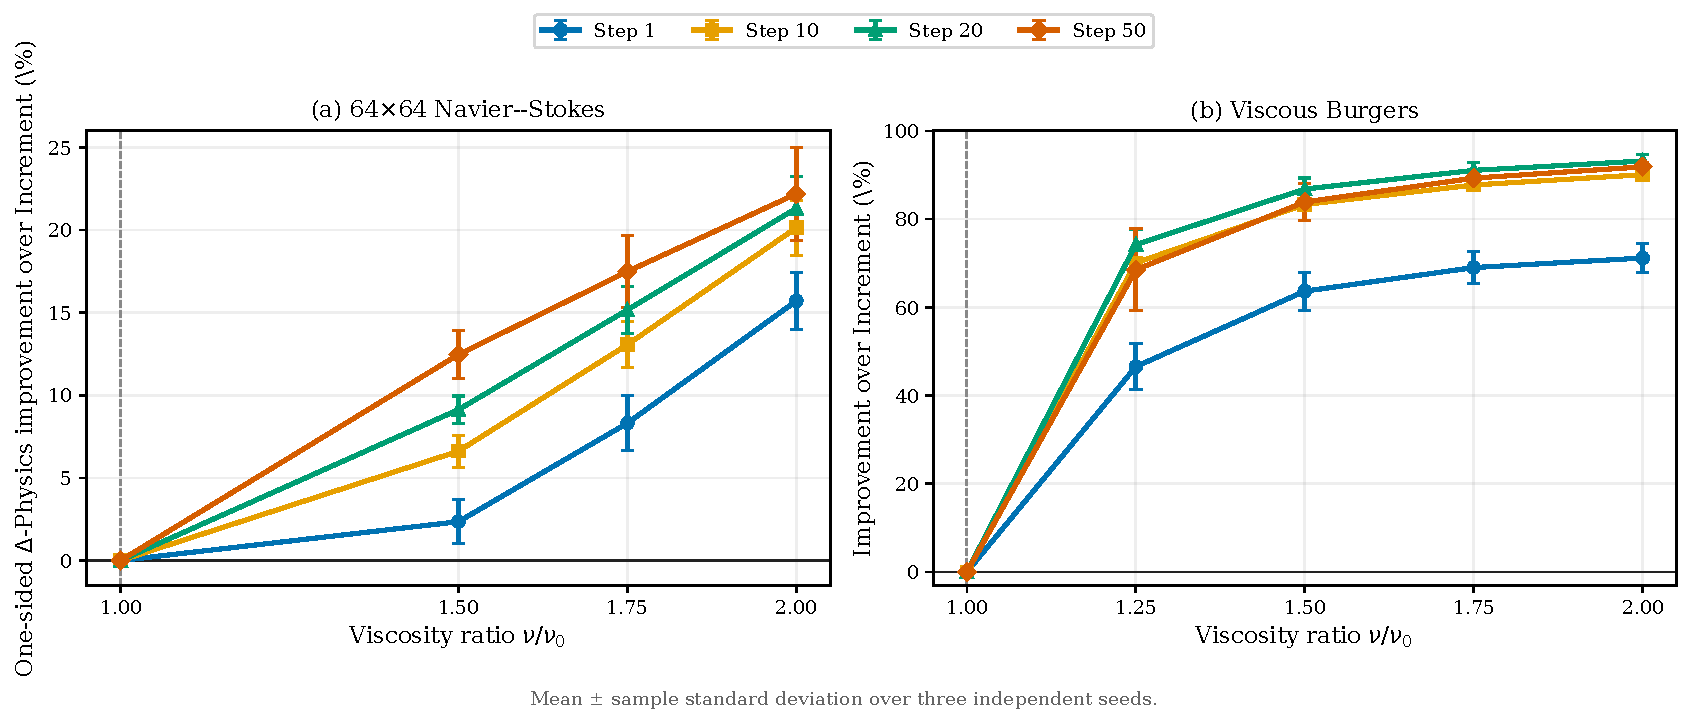
\includegraphics[width=\textwidth]{figure_2_cross_pde_improvement.pdf}
    \caption{Relative RelL2 improvement of One-sided $\Delta$-Physics over the
    frozen Increment predictor on (a) $64\times64$ Navier--Stokes and
    (b) viscous Burgers. Error bars show the mean $\pm$ sample standard
    deviation over three independently trained seeds. The panels use separate
    vertical ranges so that the Navier--Stokes horizon separation remains
    visible.}
    \label{fig:cross_pde}
\end{figure*}

\begin{table*}[!t]
\centering
\normalsize
\setlength{\tabcolsep}{3pt}
\renewcommand{\arraystretch}{1.17}
\begin{tabular}{@{}rlcccc@{}}
\toprule
$\nu/\nu_0$ & Method & \shortstack{Step-50\\RelL2} & \shortstack{Avg-50\\RelL2} & \shortstack{Avg-50\\PSRE} & Final PSRE \\
\midrule
\multicolumn{6}{l}{\textit{Single-$\nu$, zero-shot}} \\
1.0 & Increment & $0.4091\pm0.0611$ & $0.1965\pm0.0253$ & $0.0408\pm0.0109$ & $0.0722\pm0.0114$ \\
1.0 & $\Delta$-Physics & $0.4091\pm0.0611$ & $0.1965\pm0.0253$ & $0.0408\pm0.0109$ & $0.0722\pm0.0114$ \\
1.0 & Recast-style & $0.4091\pm0.0611$ & $0.1965\pm0.0253$ & $0.0408\pm0.0109$ & $0.0722\pm0.0114$ \\
\addlinespace[3pt]
1.5 & Increment & $0.4331\pm0.0638$ & $0.2061\pm0.0257$ & $0.0646\pm0.0266$ & $0.1317\pm0.0476$ \\
1.5 & $\Delta$-Physics & $0.3796\pm0.0612$ & $0.1845\pm0.0242$ & $0.0387\pm0.0082$ & $0.0680\pm0.0063$ \\
1.5 & Recast-style & $0.3780\pm0.0613$ & $0.1841\pm0.0242$ & $0.0385\pm0.0080$ & $0.0675\pm0.0060$ \\
\addlinespace[3pt]
1.75 & Increment & $0.4511\pm0.0657$ & $0.2157\pm0.0264$ & $0.0927\pm0.0289$ & $0.1914\pm0.0551$ \\
1.75 & $\Delta$-Physics & $0.3728\pm0.0621$ & $0.1814\pm0.0241$ & $0.0380\pm0.0072$ & $0.0667\pm0.0045$ \\
1.75 & Recast-style & $0.3709\pm0.0621$ & $0.1809\pm0.0241$ & $0.0377\pm0.0069$ & $0.0660\pm0.0044$ \\
\addlinespace[3pt]
2.0 & Increment & $0.4721\pm0.0680$ & $0.2275\pm0.0275$ & $0.1231\pm0.0310$ & $0.2558\pm0.0625$ \\
2.0 & $\Delta$-Physics & $0.3682\pm0.0632$ & $0.1792\pm0.0242$ & $0.0376\pm0.0064$ & $0.0660\pm0.0031$ \\
2.0 & Recast-style & $0.3659\pm0.0630$ & $0.1786\pm0.0242$ & $0.0372\pm0.0060$ & $0.0652\pm0.0031$ \\
\midrule
\multicolumn{6}{l}{\textit{Multi-$\nu$, supervised (target viscosities included)}} \\
1.0 & Cond. F-FNO & $0.0616\pm0.0055$ & $0.0350\pm0.0039$ & $0.0102\pm0.0037$ & $0.0213\pm0.0074$ \\
\addlinespace[3pt]
1.5 & Cond. F-FNO & $0.0492\pm0.0059$ & $0.0273\pm0.0029$ & $0.0079\pm0.0024$ & $0.0165\pm0.0062$ \\
\addlinespace[3pt]
1.75 & Cond. F-FNO & $0.0480\pm0.0038$ & $0.0264\pm0.0019$ & $0.0070\pm0.0009$ & $0.0156\pm0.0042$ \\
\addlinespace[3pt]
2.0 & Cond. F-FNO & $0.0494\pm0.0011$ & $0.0272\pm0.0008$ & $0.0066\pm0.0003$ & $0.0150\pm0.0027$ \\
\bottomrule
\end{tabular}
\caption{Main 64$\times$64 Navier--Stokes results (mean $\pm$ sample standard deviation over three seeds). Supervision regimes are shown explicitly: the zero-shot methods use only $\nu_0$, whereas Conditioned F-FNO uses five viscosities including all test values. Abbreviations: $\Delta$-Physics denotes One-sided $\Delta$-Physics; Recast-style denotes Equation-Recast-style; Cond. F-FNO denotes Conditioned F-FNO.}
\label{tab:ns64_main}
\end{table*}


At the reference viscosity, the two methods are identical by construction.
For all three seeds, the complete 50-step rollout produced by
One-sided $\Delta$-Physics at $\nu=\nu_0$ is elementwise identical to the
Increment baseline. This empirically verifies the exact baseline-recovery
property derived in Section~\ref{sec:reference_recovery}.

For higher viscosities, the correction produces increasingly large gains.
At $\nu/\nu_0=1.5$, the Step-50 RelL2 improvement is
$12.46\pm1.44\%$. This increases to
$17.49\pm2.17\%$ at $\nu/\nu_0=1.75$ and
$22.19\pm2.82\%$ at $\nu/\nu_0=2$.
The same monotonic trend is observed for the average rollout error.
The improvement also increases with rollout horizon. At
$\nu/\nu_0=2$, the RelL2 improvement grows from
$15.71\pm1.72\%$ at Step 1 to
$20.14\pm1.66\%$ at Step 10,
$21.31\pm1.94\%$ at Step 20, and
$22.19\pm2.82\%$ at Step 50.
The corresponding Avg-50 improvement is
$21.33\pm2.27\%$.
Thus, the benefit is not limited to an isolated one-step correction, rather, it
persists and becomes more pronounced under autoregressive rollout.

The absolute errors show the same behavior. At $\nu/\nu_0=2$, the
Increment model has Step-50 RelL2
$0.47211 \pm 0.06797$,
whereas One-sided $\Delta$-Physics reduces it to
$0.36816 \pm 0.06317$.
Avg-50 RelL2 decreases from
$0.22754 \pm 0.02750$
to
$0.17915 \pm 0.02419$.
An informative additional pattern is that the uncorrected Increment model
becomes less accurate as the target viscosity moves away from the training
viscosity, whereas the corrected model is substantially less sensitive to
this shift. For example, the Increment Avg-50 RelL2 increases from
$0.20605$ at $\nu/\nu_0=1.5$ to $0.22754$ at
$\nu/\nu_0=2$, while the corrected error decreases from
$0.18445$ to $0.17915$. This behavior is consistent with the correction
removing a viscosity-dependent dissipative mismatch rather than merely acting
as a generic rollout regularizer.

The spectral metrics strengthen this interpretation. At
$\nu/\nu_0=2$, Avg-50 PSRE decreases from
$0.12306\pm0.03099$ for Increment to
$0.03757\pm0.00636$ with One-sided $\Delta$-Physics, while final-step
PSRE decreases from
$0.25576\pm0.06247$ to
$0.06598\pm0.00310$.
The substantially larger spectral improvement indicates that the analytical
branch directly corrects a major component of the viscosity-dependent
spectral mismatch.

\subsection{Generalization to Viscous Burgers}
\label{sec:burgers_results}

We next test whether the same correction principle transfers to a different
PDE and a different neural-operator backbone. Figure~\ref{fig:cross_pde}(b)
and Table~\ref{tab:burgers_main} report the Burgers results, while the full
horizon-wise metrics are provided in
Table~\ref{tab:burgers_absolute}.

\begin{table*}[!t]
\centering
\normalsize
\setlength{\tabcolsep}{3pt}
\renewcommand{\arraystretch}{1.17}
\begin{tabular}{@{}rlcccc@{}}
\toprule
$\nu/\nu_0$ & Method & \shortstack{Step-50\\RelL2} & \shortstack{Avg-50\\RelL2} & \shortstack{Avg-50\\PSRE} & Final PSRE \\
\midrule
1.0 & Increment & $0.0517\pm0.0115$ & $0.0305\pm0.0038$ & $0.0233\pm0.0116$ & $0.0445\pm0.0220$ \\
1.0 & $\Delta$-Physics & $0.0517\pm0.0115$ & $0.0305\pm0.0038$ & $0.0233\pm0.0116$ & $0.0445\pm0.0220$ \\
\addlinespace[3pt]
1.25 & Increment & $0.1390\pm0.0339$ & $0.0898\pm0.0162$ & $0.0985\pm0.0330$ & $0.1741\pm0.0811$ \\
1.25 & $\Delta$-Physics & $0.0425\pm0.0125$ & $0.0255\pm0.0053$ & $0.0227\pm0.0108$ & $0.0444\pm0.0210$ \\
\addlinespace[3pt]
1.5 & Increment & $0.2618\pm0.0669$ & $0.1691\pm0.0306$ & $0.2172\pm0.0818$ & $0.3984\pm0.2204$ \\
1.5 & $\Delta$-Physics & $0.0409\pm0.0098$ & $0.0248\pm0.0047$ & $0.0227\pm0.0091$ & $0.0438\pm0.0198$ \\
\addlinespace[3pt]
1.75 & Increment & $0.3990\pm0.1130$ & $0.2529\pm0.0494$ & $0.3679\pm0.1626$ & $0.7107\pm0.4501$ \\
1.75 & $\Delta$-Physics & $0.0417\pm0.0089$ & $0.0251\pm0.0035$ & $0.0234\pm0.0071$ & $0.0441\pm0.0176$ \\
\addlinespace[3pt]
2.0 & Increment & $0.5507\pm0.1721$ & $0.3411\pm0.0737$ & $0.5608\pm0.2912$ & $1.1645\pm0.8532$ \\
2.0 & $\Delta$-Physics & $0.0444\pm0.0120$ & $0.0259\pm0.0026$ & $0.0248\pm0.0049$ & $0.0466\pm0.0140$ \\
\bottomrule
\end{tabular}
\caption{Main viscous Burgers results (mean $\pm$ sample standard deviation over three seeds). $\Delta$-Physics denotes One-sided $\Delta$-Physics.}
\label{tab:burgers_main}
\end{table*}


The qualitative behavior observed on Navier--Stokes transfers directly to
Burgers, but the magnitude of the gains is substantially larger. At
$\nu=\nu_0$, the corrected and uncorrected rollouts again coincide exactly.
For every higher viscosity and every evaluated rollout horizon,
One-sided $\Delta$-Physics improves over the Increment FNO.

At $\nu/\nu_0=1.25$, the Step-1 improvement is already
$46.56\pm5.24\%$, while the Avg-50 improvement reaches
$71.20\pm6.09\%$. Increasing the viscosity ratio to $1.5$, $1.75$, and
$2.0$ raises the Avg-50 improvement to
$85.07\pm3.38\%$,
$89.87\pm2.04\%$, and
$92.23\pm1.28\%$, respectively.
At $\nu/\nu_0=2$, Step-50 RelL2 improves by
$91.87\pm0.92\%$.

The absolute rollout errors reveal an especially clear separation between the
two methods. At $\nu/\nu_0=2$, the Increment model has Avg-50 RelL2
$0.34107 \pm 0.07368$,
whereas One-sided $\Delta$-Physics reduces this value to
$0.02593 \pm 0.00262$.
The Step-50 error similarly decreases from
$0.55071 \pm 0.17208$
to
$0.04437 \pm 0.01199$.

Notably, the corrected Avg-50 RelL2 remains close to
$0.025$--$0.026$ throughout the range
$\nu/\nu_0\in[1.25,2]$, even though the uncorrected Increment error increases
from $0.08981$ to $0.34107$. The same stabilization is visible in the
frequency domain. At $\nu/\nu_0=2$, Avg-50 PSRE decreases from
$0.56080\pm0.29116$ to $0.02484\pm0.00492$, and final PSRE decreases
from $1.16447\pm0.85319$ to $0.04655\pm0.01401$.

These results are important for two reasons. First, they show that the
Navier--Stokes results are not specific to a particular flow configuration.
Second, the correction is applied to a standard one-dimensional FNO rather
than the F-FNO used for Navier--Stokes. The same analytical formula therefore
produces the same qualitative parameter-shift behavior across two PDEs and
two Fourier neural-operator backbones.

\subsection{Spectral Mechanism}
\label{sec:spectral_analysis}

The form of the correction suggests that its primary effect should appear in
the spectral distribution of the predicted state. We examine this directly in
Figure~\ref{fig:spectrum} for $64\times64$ Navier--Stokes at
$\nu/\nu_0=2$ and rollout Step 50. The figure pools 24 test trajectories
across the three independent seeds.

\begin{figure*}[t]
    \centering
    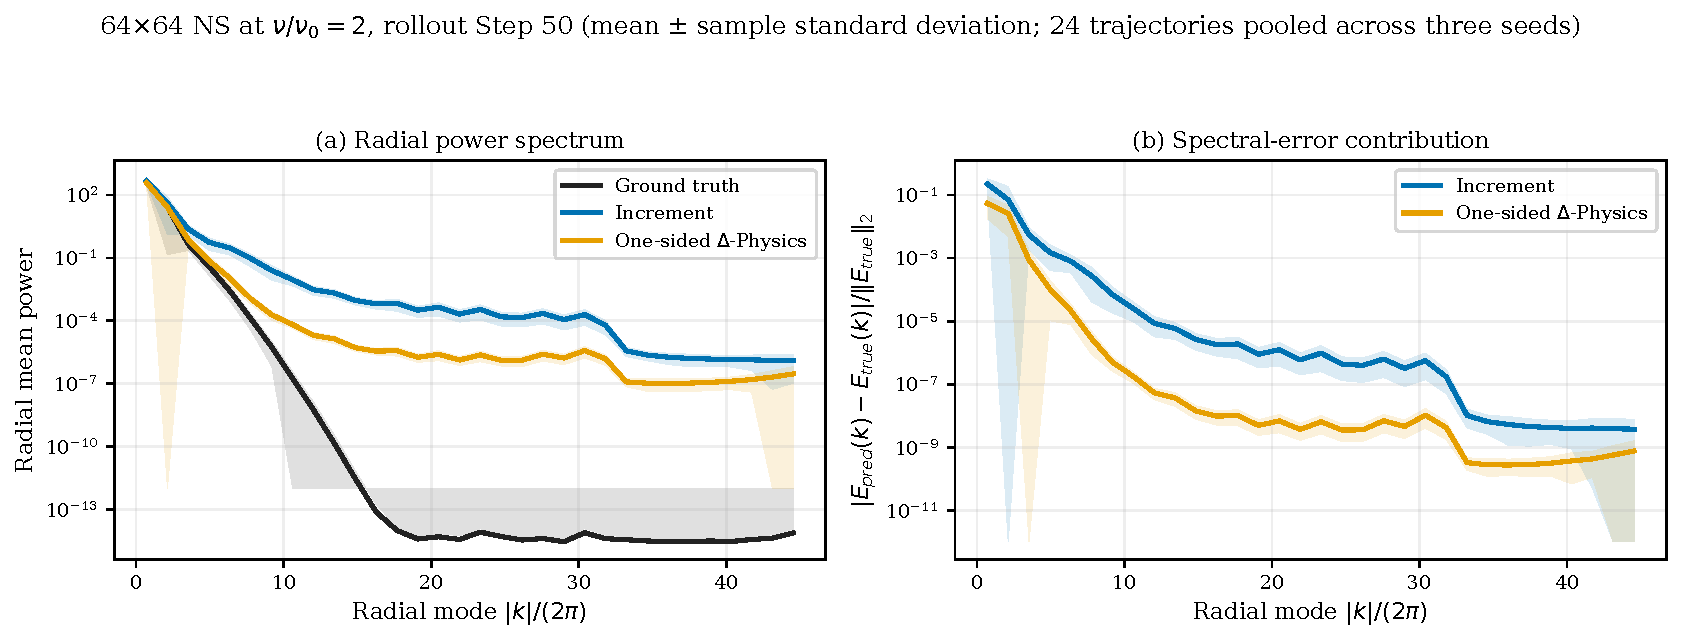
\includegraphics[width=\textwidth]{figure_3_ns_spectral_mechanism.pdf}
    \caption{Spectral mechanism on $64\times64$ Navier--Stokes at
    $\nu/\nu_0=2$ and rollout Step 50. (a) Radial mean power spectrum.
    (b) Per-bin contribution to spectral error. Lines and bands denote mean
    $\pm$ sample standard deviation over 24 trajectories pooled across the
    three seeds. The F-FNO uses factorized per-axis modes; no radial cutoff is
    implied by its mode count.}
    \label{fig:spectrum}
\end{figure*}

Figure~\ref{fig:spectrum}(a) shows the radial power spectrum. The frozen
Increment model retains substantially more spectral power than the ground
truth over a broad range of nonzero modes, consistent with a model that was
trained at a lower viscosity and therefore underestimates the amount of
dissipation required at the target parameter. One-sided $\Delta$-Physics
suppresses this excess power and shifts the predicted spectrum toward the
more strongly dissipated target spectrum.

Figure~\ref{fig:spectrum}(b) shows the corresponding spectral-error
contribution as a function of radial mode. The corrected rollout exhibits
lower error over almost the entire resolved spectral range, with particularly
large reductions away from the lowest modes. This behavior is consistent with
the stronger relative attenuation of higher-frequency modes under the target
dissipative semigroup, since
\begin{equation}
    \frac{S_\nu(\mathbf{k})}{S_{\nu_0}(\mathbf{k})}
    = \exp[-(\nu-\nu_0)|\mathbf{k}|^2\Delta t]
\end{equation}
decreases with $|\mathbf{k}|$ for $\nu>\nu_0$. The absolute magnitude of the
semigroup difference in Eq.~\eqref{eq:delta_fourier} is not monotone in
frequency; both multipliers approach zero at sufficiently high frequencies.

Together with the PSRE results in
Tables~\ref{tab:ns64_main} and~\ref{tab:burgers_main}, the spectral analysis
supports the intended mechanism of $\Delta$-Physics. The improvement is a 
reduction in aggregate state-space error accompanied by a
systematic correction of the viscosity-dependent spectral-energy mismatch.

\subsection{Comparison with Alternative Adaptation Regimes}
\label{sec:alternative_baselines}

The previous experiments compare One-sided $\Delta$-Physics with its frozen
single-viscosity Increment backbone. We next ask whether a more expensive
adaptation strategy can achieve better accuracy, and what resources are
required to do so. We consider two complementary baselines:
a fully supervised multi-viscosity conditioned F-FNO and an
Equation-Recast-style iterative zero-shot method.
The resulting accuracy--cost tradeoff is summarized in
Figure~\ref{fig:tradeoff} and Table~\ref{tab:data_compute}.

\begin{figure*}[t]
    \centering
    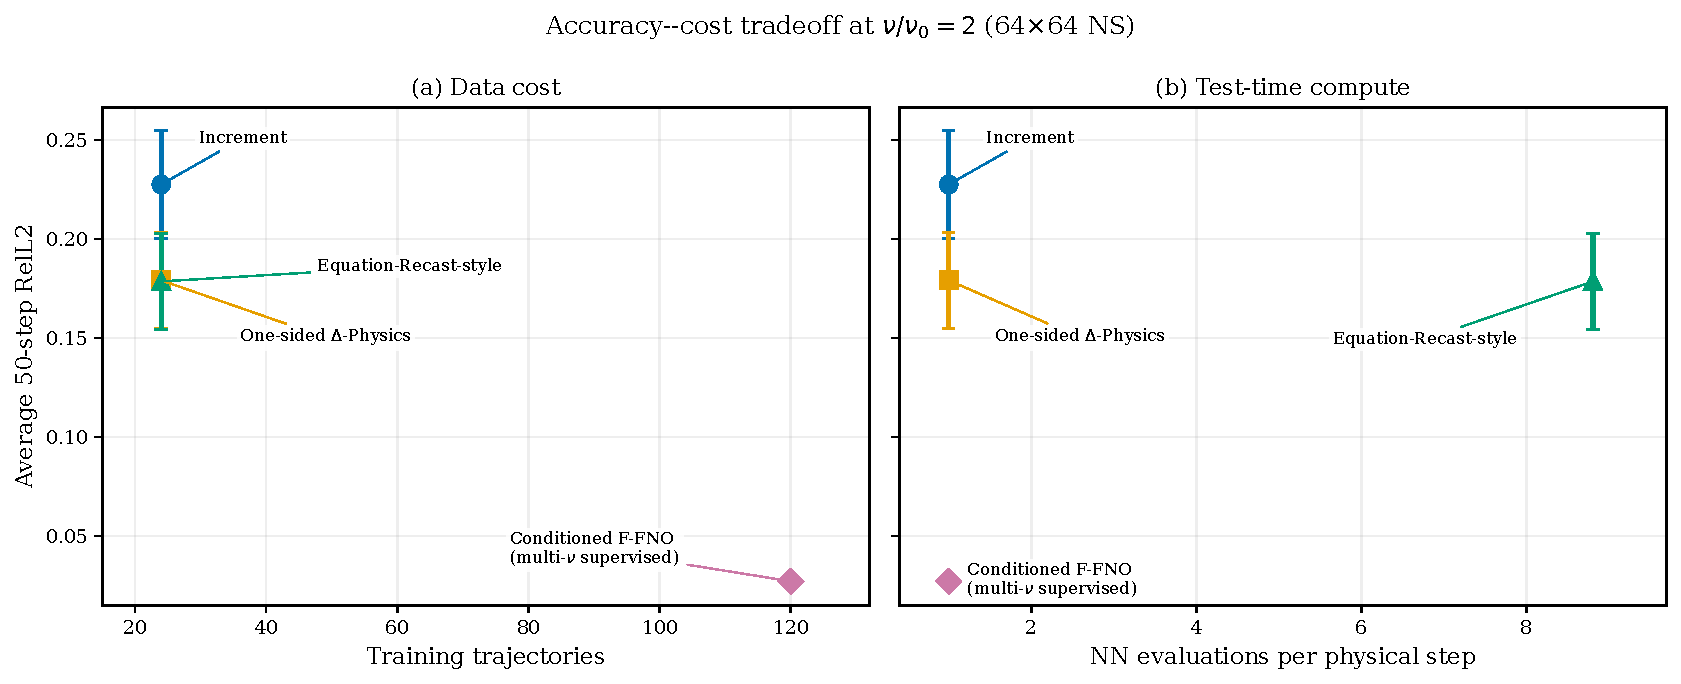
\includegraphics[width=\textwidth]{figure_4_accuracy_cost.pdf}
    \caption{Accuracy--resource tradeoff on $64\times64$ Navier--Stokes at
    $\nu/\nu_0=2$. (a) Number of training trajectories. (b) Neural-network
    evaluations per physical step. Conditioned F-FNO is a multi-viscosity
    supervised model; the remaining methods reuse a single-viscosity
    checkpoint.}
    \label{fig:tradeoff}
\end{figure*}

\begin{table*}[!t]
\centering
\normalsize
\setlength{\tabcolsep}{3pt}
\renewcommand{\arraystretch}{1.17}
\begin{tabular}{@{}lccccc@{}}
\toprule
Method & \shortstack{Train\\trajectories} & \shortstack{Train\\pairs} & \shortstack{Optimizer\\time (s)} & \shortstack{NN evals\\/ step} & \shortstack{Inference\\time (s)} \\
\midrule
Increment & 24 & 480 & 280.19 $\pm$ 2.92 & 1.00 & 7.53 $\pm$ 0.83 \\
$\Delta$-Physics & 24 & 480 & 280.19 $\pm$ 2.92 & 1.00 & 8.06 $\pm$ 1.40 \\
Recast-style & 24 & 480 & 280.19 $\pm$ 2.92 & 8.81 & 70.08 $\pm$ 8.50 \\
Cond. F-FNO & 120 & 2400 & 1275.70 $\pm$ 86.78 & 1.00 & 7.38 $\pm$ 0.32 \\
\bottomrule
\end{tabular}
\caption{Data and compute comparison. Inference time is measured on CPU for one viscosity, eight trajectories, and 50 rollout steps at $\nu/\nu_0=2$. One-sided Delta-Physics and Equation-Recast-style reuse the Increment checkpoint and require no additional training. Abbreviations: $\Delta$-Physics denotes One-sided $\Delta$-Physics; Recast-style denotes Equation-Recast-style; Cond. F-FNO denotes Conditioned F-FNO. The first three methods use one training viscosity and 28,370 parameters, with no target-parameter training data; Cond. F-FNO uses five viscosities, target-parameter training data, and 28,386 parameters. Optimizer time excludes data generation.}
\label{tab:data_compute}
\end{table*}


\paragraph{Multi-viscosity conditioned F-FNO.}
The conditioned baseline uses the same F-FNO width, number of modes, depth,
optimizer, number of epochs, and number of trajectories per viscosity as the
single-viscosity model. In addition to the normalized state and spatial
coordinates, it receives
\begin{equation}
    q
    =
    \frac{
        \log(\nu/\nu_0)-\mu_q
    }{
        \sigma_q
    }
    \label{eq:conditioned_q}
\end{equation}
as a spatially constant input channel. It is trained jointly on
\begin{equation}
    \frac{\nu}{\nu_0}
    \in
    \{1.0,1.25,1.5,1.75,2.0\}.
\end{equation}
Thus, unlike One-sided $\Delta$-Physics, this baseline is not zero-shot at the
reported target viscosities: all evaluated viscosities are covered during
training.

As expected, access to target-parameter trajectories provides a large
accuracy advantage. At $\nu/\nu_0=2$, the conditioned model achieves
Avg-50 RelL2
$    0.02716 \pm 0.00076,
$
compared with
$    0.17915 \pm 0.02419$
for single-viscosity One-sided $\Delta$-Physics. Step-50 RelL2 is
$0.04941\pm0.00109$ for the conditioned model and
$0.36816\pm0.06317$ for $\Delta$-Physics.
The conditioned model is therefore the preferable accuracy-oriented choice
when simulations at the target parameter range are available.

However, the supervision requirements are substantially different.
One-sided $\Delta$-Physics uses 24 training trajectories from a single
viscosity, corresponding to 480 one-step training pairs. The conditioned
model uses 24 trajectories at each of five viscosities, for a total of
120 trajectories and 2,400 training pairs. Its parameter count increases only
slightly, from 28,370 to 28,386, showing that its additional cost is primarily
in parameter-space data coverage and optimization rather than model size.
In our timing experiment, optimizer time increases from
$280.19\pm2.92$ seconds per seed for the single-viscosity model to
$1275.70\pm86.78$ seconds for the conditioned model, a factor of
approximately $4.55$.

This comparison demonstrates that
multi-viscosity conditioning is substantially more accurate when
target-parameter simulations are available, whereas One-sided
$\Delta$-Physics provides adaptation without requiring any such simulations
or retraining.

\paragraph{Equation-Recast-style iterative baseline.}
We also compare against an iterative zero-shot baseline inspired by operator
recasting. Because the frozen model in our setting is a state-to-state
time-stepper rather than a steady source-to-solution inverse, we use a dynamic
backward-Euler interpretation rather than treating this baseline as an exact
reproduction of the original steady formulation.

Given the current physical state $u_t$, we initialize
\begin{equation}
    y^{(0)}
    =
    \Phi_{\theta,\nu_0}(u_t)
\end{equation}
and define the fixed-point map
\begin{equation}
    G_\nu(y;u_t)
    =
    \Phi_{\theta,\nu_0}
    \left(
        u_t
        +
        \Delta t(\nu-\nu_0)\Delta y
    \right).
    \label{eq:dynamic_recast}
\end{equation}
We apply vector Aitken relaxation to the residual
\begin{equation}
    r^{(k)}
    =
    G_\nu(y^{(k)};u_t)-y^{(k)}
\end{equation}
and iterate until the relative fixed-point residual is below $10^{-5}$,
with a maximum of 30 iterations. At $\nu=\nu_0$, the method explicitly
reduces to a single evaluation of the Increment model.

The iterative solver is numerically stable in the tested high-viscosity
regime. Across all 3,600 OOD trajectory-step evaluations, no non-converged
step or NaN/Inf event is observed. At $\nu/\nu_0=2$, it requires
$7.81$ iterations on average, corresponding to $8.81$ neural-network
evaluations per physical step. Further convergence statistics are reported in
Table~\ref{tab:recast_convergence}.

Despite this additional computation, its accuracy improvement over
One-sided $\Delta$-Physics is small. At $\nu/\nu_0=2$, Equation-Recast-style
improves Avg-50 RelL2 over $\Delta$-Physics by only
$0.31\pm0.09\%$ and Step-50 RelL2 by
$0.62\pm0.10\%$. The corresponding absolute Avg-50 errors are
$0.17859\pm0.02418$ and $0.17915\pm0.02419$, respectively.

The computational difference is much larger. As shown in
Figure~\ref{fig:tradeoff}(b), One-sided $\Delta$-Physics retains exactly one
neural-network evaluation per physical step, whereas the iterative baseline
requires $8.81$ evaluations per step at $\nu/\nu_0=2$. Measured inference
time increases from $8.06\pm1.40$ seconds to
$70.08\pm8.50$ seconds under the same evaluation setting.
Thus, the iterative refinement recovers only a small additional accuracy gain
while increasing inference cost by approximately an order of magnitude.

Figure~\ref{fig:tradeoff} summarizes the complementary tradeoffs.
Figure~\ref{fig:tradeoff}(a) shows that the conditioned F-FNO achieves the
lowest error but requires five times as many training trajectories, while
Figure~\ref{fig:tradeoff}(b) shows that Equation-Recast-style reaches nearly
the same accuracy as One-sided $\Delta$-Physics but with substantially greater
test-time computation. One-sided $\Delta$-Physics occupies the regime with
single-viscosity supervision, no additional learned parameters, no
retraining, and one neural-network evaluation per physical step.

\subsection{Why One-Sided?}
\label{sec:onesided_ablation}

The main experiments focus on $\nu\ge\nu_0$, for which the semigroup
difference is dissipative. To examine whether the same correction can be
applied symmetrically to lower viscosities, we additionally perform a dense
no-retraining viscosity scan using the untruncated two-sided correction.
Results are shown in Appendix Figure~\ref{fig:two_sided}.

The scan covers
\begin{equation}
    \frac{\nu}{\nu_0}
    \in
    \{
    0.5,\,
    0.625,\,
    0.75,\,
    0.875,\,
    1.0,\,
    1.25,\,
    1.5,\,
    1.75,\,
    2.0
    \}.
\end{equation}
The high-viscosity side reproduces the monotonic improvement observed in the
formal three-seed experiments. The low-viscosity side behaves differently.
For $\nu<\nu_0$, the correction can improve short-horizon prediction, but the
benefit reverses as the rollout becomes longer.

The most extreme case occurs at $\nu/\nu_0=0.5$: Step-1 RelL2 improves by
$10.53\%$, but the improvement becomes negative by Step 20 and reaches
$-296.76\%$ at Step 50. The Step-50 deterioration is also substantial at
ratios $0.625$, $0.75$, and $0.875$, where the relative changes are
$-52.29\%$, $-14.53\%$, and $-5.06\%$, respectively.
Figure~\ref{fig:two_sided}(b) shows that this reversal emerges progressively
as the target viscosity moves below the reference value.

This asymmetry is consistent with the analysis in
Section~\ref{sec:dissipative_property}. For $\nu>\nu_0$, the correction
supplies additional dissipation and has a non-positive Fourier multiplier.
For $\nu<\nu_0$, the multiplier reverses sign, so repeatedly applying the
correction acts in an anti-dissipative direction. While such a correction may
reduce the immediate one-step mismatch, it can amplify spectral and state
errors under autoregressive recursion.

We therefore adopt the one-sided policy used throughout the main experiments:
the analytical correction is activated only for $\nu>\nu_0$, while the
frozen Increment predictor is retained unchanged for $\nu\le\nu_0$.


\paragraph{Sensitivity to reference training budget.}
To examine whether the gains arise primarily from an
undertrained reference model, we conduct an additional
training-budget sensitivity study using the same 24
reference-viscosity trajectories and random seed, extending
training from 15 to 75 epochs. The reference-viscosity
Increment Step-50 RelL2 decreases substantially from
$0.37282$ to $0.09452$. Nevertheless, at
$\nu/\nu_0=2$, One-sided $\Delta$-Physics further reduces
the stronger model's Avg-50 RelL2 from $0.12423$ to
$0.04634$, a $62.70\%$ improvement, and Step-50 RelL2
from $0.21283$ to $0.07819$, a $63.26\%$
improvement. These results indicate that the analytical
correction remains effective for a substantially more
accurate reference time-stepper. Full single-seed
results are provided in Appendix~\ref{sec:training_budget}.



\section{Conclusion}
\label{sec:conclusion}

We presented One-sided $\Delta$-Physics, a simple
analytical framework for zero-shot adaptation of
pretrained neural PDE time-steppers to unseen
higher viscosities. By exploiting the known
dependence of linear dissipative dynamics on
viscosity, the method corrects a frozen reference
prediction through the difference between
dissipative semigroups. The one-sided construction
provides an additional dissipative correction
while avoiding potentially harmful anti-dissipative
adjustments. Importantly, the method requires
no retraining, additional learned parameters,
or iterative neural inference, and exactly
preserves the reference predictor at the
training viscosity.

Experiments on two-dimensional Navier--Stokes
and one-dimensional viscous Burgers equations
demonstrated consistent improvements in
long-horizon prediction and spectral accuracy
under unseen higher-viscosity conditions.
The improvements generally increased with
viscosity shift and rollout horizon, while
spectral analysis supported the intended
dissipative correction mechanism.
Comparisons with alternative adaptation
strategies further clarified the tradeoffs:
multi-viscosity supervised learning achieved
higher accuracy when target-parameter data
were available, whereas iterative zero-shot
adaptation provided only marginal additional
accuracy at substantially greater inference cost.

The present framework has several limitations.
Its analytical correction relies on a known
linear dissipative operator and is currently
validated primarily for periodic diffusion
with viscosity shifts toward stronger
dissipation. It does not explicitly correct
changes in nonlinear dynamics, nor does
the dissipative property of the correction
guarantee global stability of the complete
neural rollout. Future work could extend
the framework to more general dissipative
operators, boundary conditions, and physical
parameters, and investigate how analytical
corrections can be combined with learned
models of nonlinear parameter dependence.



\bibliographystyle{unsrt}
\bibliography{references}

\clearpage
\onecolumn
\appendix
\section{Why the Final Policy Is One-Sided}
\label{sec:one_sided_ablation}
Figure~\ref{fig:two_sided} reports the dense viscosity sweep used to select the
one-sided policy. A two-sided semigroup-difference correction helps at early
steps for $\nu<\nuRef$, but the long-horizon benefit reverses and becomes
strongly negative as viscosity decreases. In contrast, the high-viscosity side
improves consistently with shift and horizon.

\begin{figure}[!htbp]
    \centering
    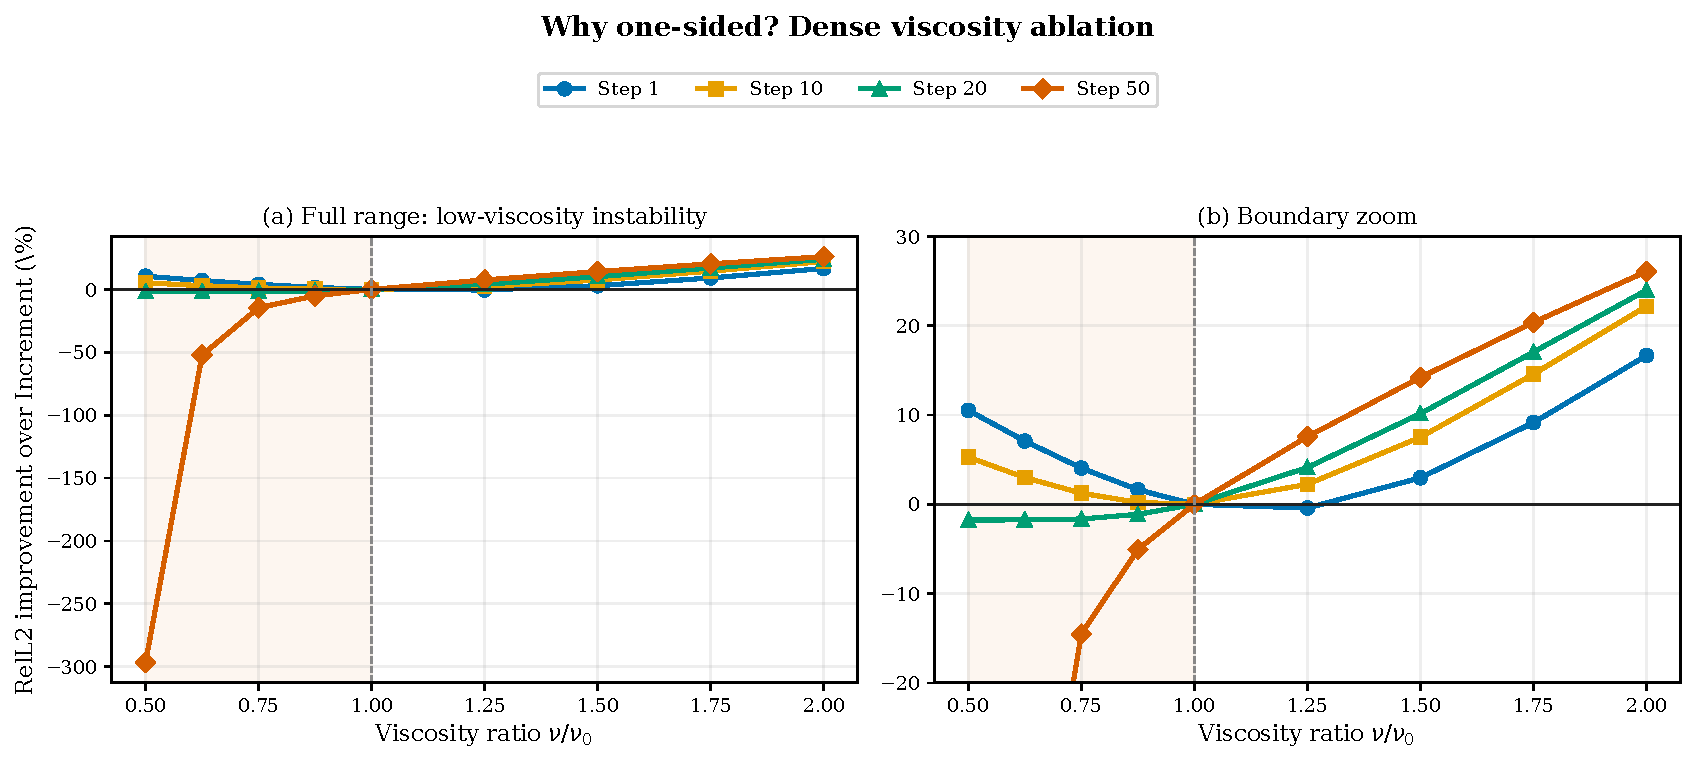
\includegraphics[width=\textwidth]{figure_s1_dense_two_sided_ablation.pdf}
    \caption{Dense two-sided viscosity ablation. The full range (left) exposes
    low-viscosity long-rollout instability; the boundary zoom (right) shows the
    transition around $\nu=\nuRef$. This motivates the hard one-sided policy.}
    \label{fig:two_sided}
\end{figure}

\section{Equation-Recast-Style Convergence}
The iterative baseline converges for every evaluated trajectory-step, but its
mean number of neural evaluations rises with viscosity shift. This produces
only a marginal accuracy improvement over the single-pass correction at a
substantially higher inference cost.

\begin{table*}[!htbp]
\centering
\small
\resizebox{\textwidth}{!}{%
\begin{tabular}{rlccccc}
\toprule
nu/nu0 & Mean iterations & P95 iterations & Max iterations & Mean NN evals / step & Non-converged steps & Inference time (s) \\
\midrule
1.0 & 0.00 & 0.0 & 0 & 1.00 & 0 & 7.32 $\pm$ 1.52 \\
1.5 & 5.86 & 6.0 & 6 & 6.86 & 0 & 48.22 $\pm$ 3.29 \\
1.75 & 6.41 & 7.0 & 8 & 7.41 & 0 & 61.20 $\pm$ 5.16 \\
2.0 & 7.81 & 8.0 & 9 & 8.81 & 0 & 70.08 $\pm$ 8.50 \\
\bottomrule
\end{tabular}%
}
\caption{Equation-Recast-style fixed-point diagnostics at tolerance $10^{-5}$ and at most 30 iterations. Counts pool three seeds, eight trajectories, and 50 physical steps per viscosity.}
\label{tab:recast_convergence}
\end{table*}


\clearpage
\section{Full-Horizon Tables}
The following tables retain the complete Step-1/10/20/50 results used to create
the main figures.

\subsection{Navier--Stokes}
\begin{table*}[!htbp]
\centering
\small
\setlength{\tabcolsep}{4pt}
\renewcommand{\arraystretch}{1.12}
\textit{(a) Horizon-specific relative errors}\par\smallskip
\begin{tabular}{@{}rlcccc@{}}
\toprule
$\nu/\nu_0$ & Method & Step 1 RelL2 & Step 10 RelL2 & Step 20 RelL2 & Step 50 RelL2 \\
\midrule
1.0 & Increment & $0.00898\pm0.00120$ & $0.07923\pm0.01009$ & $0.14993\pm0.01717$ & $0.40913\pm0.06111$ \\
1.0 & $\Delta$-Physics & $0.00898\pm0.00120$ & $0.07923\pm0.01009$ & $0.14993\pm0.01717$ & $0.40913\pm0.06111$ \\
1.0 & Recast-style & $0.00898\pm0.00120$ & $0.07923\pm0.01009$ & $0.14993\pm0.01717$ & $0.40913\pm0.06111$ \\
1.0 & Cond. F-FNO & $0.00226\pm0.00029$ & $0.01804\pm0.00240$ & $0.03051\pm0.00410$ & $0.06163\pm0.00547$ \\
1.5 & Increment & $0.00911\pm0.00111$ & $0.08115\pm0.00937$ & $0.15581\pm0.01667$ & $0.43308\pm0.06382$ \\
1.5 & $\Delta$-Physics & $0.00890\pm0.00118$ & $0.07579\pm0.00900$ & $0.14157\pm0.01511$ & $0.37956\pm0.06122$ \\
1.5 & Recast-style & $0.00892\pm0.00117$ & $0.07578\pm0.00895$ & $0.14148\pm0.01503$ & $0.37802\pm0.06129$ \\
1.5 & Cond. F-FNO & $0.00205\pm0.00024$ & $0.01477\pm0.00157$ & $0.02357\pm0.00234$ & $0.04922\pm0.00592$ \\
1.75 & Increment & $0.00966\pm0.00113$ & $0.08564\pm0.00956$ & $0.16382\pm0.01722$ & $0.45106\pm0.06568$ \\
1.75 & $\Delta$-Physics & $0.00887\pm0.00117$ & $0.07446\pm0.00856$ & $0.13895\pm0.01451$ & $0.37283\pm0.06213$ \\
1.75 & Recast-style & $0.00889\pm0.00116$ & $0.07444\pm0.00848$ & $0.13883\pm0.01443$ & $0.37093\pm0.06211$ \\
1.75 & Cond. F-FNO & $0.00209\pm0.00020$ & $0.01454\pm0.00119$ & $0.02268\pm0.00157$ & $0.04798\pm0.00383$ \\
2.0 & Increment & $0.01047\pm0.00119$ & $0.09182\pm0.01005$ & $0.17414\pm0.01820$ & $0.47211\pm0.06797$ \\
2.0 & $\Delta$-Physics & $0.00884\pm0.00116$ & $0.07332\pm0.00818$ & $0.13697\pm0.01411$ & $0.36816\pm0.06317$ \\
2.0 & Recast-style & $0.00887\pm0.00115$ & $0.07329\pm0.00809$ & $0.13679\pm0.01404$ & $0.36589\pm0.06302$ \\
2.0 & Cond. F-FNO & $0.00223\pm0.00017$ & $0.01523\pm0.00092$ & $0.02341\pm0.00093$ & $0.04941\pm0.00109$ \\
\bottomrule
\end{tabular}\par\medskip
\textit{(b) Average rollout and spectral errors}\par\smallskip
\begin{tabular}{@{}rlccc@{}}
\toprule
$\nu/\nu_0$ & Method & Avg-50 RelL2 & Avg-50 PSRE & Final PSRE \\
\midrule
1.0 & Increment & $0.19647\pm0.02527$ & $0.04083\pm0.01086$ & $0.07224\pm0.01139$ \\
1.0 & $\Delta$-Physics & $0.19647\pm0.02527$ & $0.04083\pm0.01086$ & $0.07224\pm0.01139$ \\
1.0 & Recast-style & $0.19647\pm0.02527$ & $0.04083\pm0.01086$ & $0.07224\pm0.01139$ \\
1.0 & Cond. F-FNO & $0.03504\pm0.00394$ & $0.01019\pm0.00372$ & $0.02129\pm0.00744$ \\
1.5 & Increment & $0.20605\pm0.02567$ & $0.06463\pm0.02655$ & $0.13174\pm0.04764$ \\
1.5 & $\Delta$-Physics & $0.18445\pm0.02419$ & $0.03872\pm0.00822$ & $0.06802\pm0.00626$ \\
1.5 & Recast-style & $0.18408\pm0.02420$ & $0.03849\pm0.00800$ & $0.06749\pm0.00605$ \\
1.5 & Cond. F-FNO & $0.02733\pm0.00287$ & $0.00793\pm0.00242$ & $0.01652\pm0.00624$ \\
1.75 & Increment & $0.21566\pm0.02640$ & $0.09274\pm0.02886$ & $0.19137\pm0.05505$ \\
1.75 & $\Delta$-Physics & $0.18135\pm0.02412$ & $0.03804\pm0.00722$ & $0.06674\pm0.00454$ \\
1.75 & Recast-style & $0.18089\pm0.02412$ & $0.03773\pm0.00693$ & $0.06603\pm0.00443$ \\
1.75 & Cond. F-FNO & $0.02637\pm0.00189$ & $0.00699\pm0.00091$ & $0.01560\pm0.00420$ \\
2.0 & Increment & $0.22754\pm0.02750$ & $0.12306\pm0.03099$ & $0.25576\pm0.06247$ \\
2.0 & $\Delta$-Physics & $0.17915\pm0.02419$ & $0.03757\pm0.00636$ & $0.06598\pm0.00310$ \\
2.0 & Recast-style & $0.17859\pm0.02418$ & $0.03720\pm0.00604$ & $0.06520\pm0.00309$ \\
2.0 & Cond. F-FNO & $0.02716\pm0.00076$ & $0.00663\pm0.00034$ & $0.01505\pm0.00269$ \\
\bottomrule
\end{tabular}\par\medskip
\caption{Absolute 64$\times$64 Navier--Stokes rollout errors (mean $\pm$ sample standard deviation over three seeds). Conditioned F-FNO uses five training viscosities; the remaining methods use only $\nu_0$ training data.}
\label{tab:ns64_absolute}
\end{table*}


\clearpage
\subsection{Viscous Burgers}
\begin{table*}[!htbp]
\centering
\small
\setlength{\tabcolsep}{4pt}
\renewcommand{\arraystretch}{1.12}
\textit{(a) Horizon-specific relative errors}\par\smallskip
\begin{tabular}{@{}rlcccc@{}}
\toprule
$\nu/\nu_0$ & Method & Step 1 RelL2 & Step 10 RelL2 & Step 20 RelL2 & Step 50 RelL2 \\
\midrule
1.0 & Increment & $0.00647\pm0.00050$ & $0.01961\pm0.00133$ & $0.02566\pm0.00220$ & $0.05173\pm0.01146$ \\
1.0 & $\Delta$-Physics & $0.00647\pm0.00050$ & $0.01961\pm0.00133$ & $0.02566\pm0.00220$ & $0.05173\pm0.01146$ \\
1.25 & Increment & $0.01197\pm0.00046$ & $0.05735\pm0.00489$ & $0.08260\pm0.01168$ & $0.13899\pm0.03389$ \\
1.25 & $\Delta$-Physics & $0.00638\pm0.00048$ & $0.01718\pm0.00188$ & $0.02114\pm0.00289$ & $0.04250\pm0.01252$ \\
1.5 & Increment & $0.02037\pm0.00078$ & $0.10787\pm0.01018$ & $0.15639\pm0.02190$ & $0.26181\pm0.06694$ \\
1.5 & $\Delta$-Physics & $0.00738\pm0.00062$ & $0.01797\pm0.00196$ & $0.02036\pm0.00306$ & $0.04091\pm0.00983$ \\
1.75 & Increment & $0.02910\pm0.00120$ & $0.15729\pm0.01606$ & $0.23149\pm0.03398$ & $0.39896\pm0.11298$ \\
1.75 & $\Delta$-Physics & $0.00899\pm0.00077$ & $0.01919\pm0.00176$ & $0.02036\pm0.00270$ & $0.04174\pm0.00892$ \\
2.0 & Increment & $0.03781\pm0.00166$ & $0.20551\pm0.02241$ & $0.30780\pm0.04867$ & $0.55071\pm0.17208$ \\
2.0 & $\Delta$-Physics & $0.01086\pm0.00088$ & $0.02023\pm0.00151$ & $0.02058\pm0.00204$ & $0.04437\pm0.01199$ \\
\bottomrule
\end{tabular}\par\medskip
\textit{(b) Average rollout and spectral errors}\par\smallskip
\begin{tabular}{@{}rlccc@{}}
\toprule
$\nu/\nu_0$ & Method & Avg-50 RelL2 & Avg-50 PSRE & Final PSRE \\
\midrule
1.0 & Increment & $0.03053\pm0.00381$ & $0.02331\pm0.01160$ & $0.04449\pm0.02200$ \\
1.0 & $\Delta$-Physics & $0.03053\pm0.00381$ & $0.02331\pm0.01160$ & $0.04449\pm0.02200$ \\
1.25 & Increment & $0.08981\pm0.01618$ & $0.09852\pm0.03302$ & $0.17406\pm0.08112$ \\
1.25 & $\Delta$-Physics & $0.02550\pm0.00528$ & $0.02270\pm0.01076$ & $0.04442\pm0.02102$ \\
1.5 & Increment & $0.16909\pm0.03056$ & $0.21725\pm0.08182$ & $0.39840\pm0.22043$ \\
1.5 & $\Delta$-Physics & $0.02475\pm0.00466$ & $0.02275\pm0.00912$ & $0.04384\pm0.01978$ \\
1.75 & Increment & $0.25287\pm0.04943$ & $0.36794\pm0.16264$ & $0.71065\pm0.45011$ \\
1.75 & $\Delta$-Physics & $0.02506\pm0.00350$ & $0.02345\pm0.00714$ & $0.04406\pm0.01763$ \\
2.0 & Increment & $0.34107\pm0.07368$ & $0.56080\pm0.29116$ & $1.16447\pm0.85319$ \\
2.0 & $\Delta$-Physics & $0.02593\pm0.00262$ & $0.02484\pm0.00492$ & $0.04655\pm0.01401$ \\
\bottomrule
\end{tabular}\par\medskip
\caption{Absolute viscous Burgers rollout errors (mean $\pm$ sample standard deviation over three seeds).}
\label{tab:burgers_absolute}
\end{table*}


% TODO: Replace author metadata and adapt the document class to the target venue.


\section{Sensitivity to Reference Training Budget}
\label{sec:training_budget}

We investigate whether the effectiveness of One-sided
$\Delta$-Physics depends on limited optimization of the
reference neural time-stepper. We keep the original
64$\times$64 Navier--Stokes training trajectories and
random seed fixed, and increase the reference training
budget from 15 to 75 epochs. No target-viscosity
trajectories are introduced.

The longer training budget substantially improves the
reference predictor. At $\nu=\nu_0$, its Step-50
RelL2 decreases from $0.37282$ to $0.09452$.
One-sided $\Delta$-Physics preserves this stronger
reference prediction exactly.

Table~\ref{tab:training_budget} reports the zero-shot
results obtained with the 75-epoch reference model.
The correction improves both average and final-step
rollout errors across all evaluated higher viscosities,
with larger gains at greater viscosity shifts.

\begin{table}[t]
\centering
\small
\setlength{\tabcolsep}{7pt}
\caption{
Zero-shot adaptation using a more extensively trained
reference F-FNO (75 epochs, seed 0). The same 24
reference-viscosity training trajectories are used.
Improvements are relative error reductions over
the frozen Increment baseline.
}
\label{tab:training_budget}
\begin{tabular}{c r r r r r r}
\toprule
& \multicolumn{3}{c}{Avg-50 RelL2}
& \multicolumn{3}{c}{Step-50 RelL2} \\
\cmidrule(lr){2-4}
\cmidrule(lr){5-7}
$\nu/\nu_0$
& Increment
& $\Delta$-Physics
& Gain (\%)
& Increment
& $\Delta$-Physics
& Gain (\%) \\
\midrule
1.00 & 0.05609 & 0.05609 & 0.00
     & 0.09452 & 0.09452 & 0.00 \\
1.50 & 0.08028 & 0.04921 & 38.70
     & 0.13899 & 0.08232 & 40.77 \\
1.75 & 0.10145 & 0.04753 & 53.15
     & 0.17465 & 0.07985 & 54.28 \\
2.00 & 0.12423 & 0.04634 & 62.70
     & 0.21283 & 0.07819 & 63.26 \\
\bottomrule
\end{tabular}
\end{table}

At $\nu/\nu_0=2$, the corresponding Avg-50
and final-step PSRE improvements are $83.81\%$
and $84.86\%$, respectively. Moreover, the
Avg-50 and Step-50 improvements exceed those
of the original 15-epoch checkpoint, which were
$23.94\%$ and $25.23\%$ for the same seed.

This study indicates that the benefit of analytical
viscosity correction is not confined to an
undertrained reference model. The result is
based on a single seed and is intended as a
training-budget sensitivity check rather than
a replacement for the three-seed main comparison.


\end{document}
